
% Charles McEachern
% Spring 2017

% ######################################################################

% To submit your paper:
\documentclass[draft,linenumbers]{agujournal}
\draftfalse

\usepackage{siunitx} % \num{} formatting and SI unit formatting

\usepackage[noabbrev,capitalize]{cleveref} % Automatically determine \cref type


% Define a better looking eV by moving the V slightly left
\DeclareSIUnit\electronvolt{e\hspace{-0.08em}V}
\DeclareSIUnit\keV{\kilo\electronvolt}
\DeclareSIUnit\percc{/\cm\cubed}
\DeclareSIUnit\RE{R_E}
\DeclareSIUnit\nT{\nano\tesla}
\DeclareSIUnit\nJ{\nano\joule}
\DeclareSIUnit\S{S}
\DeclareSIUnit\Mm{Mm}


% For final version.
% \documentclass{agujournal}

\journalname{JGR-Space Physics}

\begin{document}

% ######################################################################

\title{Modeling Pc4 Pulsations in Two and a Half Dimensions with Comparisons to Van Allen Probes Observations}

\authors{
    Charles McEachern\affil{1},
    Robert Lysak\affil{1},
    Ian Mann\affil{2},
    Lei Dai\affil{3}, \\
    John Wygant\affil{1},
    Aaron Breneman\affil{1}, and
    Scott Thaller\affil{1}
}

\affiliation{1}{University of Minnesota}
\affiliation{2}{University of Alberta}
\affiliation{3}{???}

\correspondingauthor{Charles McEachern}{mceachern@physics.umn.edu}

%% Keypoints, final entry on title page.

% Example:
% \begin{keypoints}
% \item	List up to three key points (at least one is required)
% \item	Key Points summarize the main points and conclusions of the article
% \item	Each must be 100 characters or less with no special characters or punctuation
% \end{keypoints}

%  List up to three key points (at least one is required)
%  Key Points summarize the main points and conclusions of the article
%  Each must be 100 characters or less with no special characters or punctuation

\begin{keypoints}
\item Key point 1
\item Key point 2
\item Key point 3
\end{keypoints}

% ######################################################################

\begin{abstract}
Field line resonances (FLRs) in the Pc4 range (\SIrange{7}{25}{\mHz}) serve to energize magnetospheric particles through drift-resonant interactions, carry energy from high to low altitude, induce currents in the magnetosphere, and scatter particles into the atmosphere. Wave structure and polarization significantly impact these behaviors. The present work showcases a new two and a half dimensional code, Tuna, ideally suited to model FLRs, with the ability to consider a broad range of azimuthal modenumbers, coupling between the poloidal, toroidal, and compressional modes, and arbitrary harmonic structure. Using Tuna, the interplay between Joule dissipation and poloidal-to-toroidal rotation is considered for Pc4 pulsations under both dayside and nightside conditions. An effort is also made to incorporate giant pulsations, a subclass of Pc4 noted for its distinctive ground signatures, into the broader Pc4 morphology. Numerical results are supplemented by a survey of 762 Pc4 pulsations using data from the Van Allen Probes, the first such survey to characterize each event by both polarization and harmonic. The combination of numerical and observational results suggests an explanation for the disparate distributions observed in poloidal and toroidal Pc4 events.
\end{abstract}

% ######################################################################

\section{Introduction}

Pc4 pulsations are magnetic pulsations with periods of a minute or two (\SIrange{7}{25}{\mHz}), corresponding to resonant oscillations of field lines with $4 \lesssim L \lesssim 7$. They are notable for their drift and drift-bounce resonant interactions with trapped energetic particles\citep{southwood_1976}, which can accelerate those particles\citep{elkington_1999} and lead to radial diffusion\citep{elkington_2003}. Giant pulsations, a subclass of Pc4 pulsation, have been a topic of particular interest for over a century, due to their large, strikingly sinusoidal waveforms\citep{brekke_1987}.

A field line resonance (FLR) in the Pc4 range is subject to three mutually-independent classifications: harmonic number, azimuthal modenumber, and polarization.

Harmonic number is a measure of FLR wavelength along the geomagnetic field line. First-harmonic FLRs are associated with drift resonance, while the second harmonic is associated with drift-bounce resonance\citep{dai_2013,poulter_1983}. The wavelength of a second-harmonic FLR is equal to the length of its magnetic field line; it exhibits two nodes (antinodes) in the magnetic (electric) perturbation, with magnentic antinodes (electric nodes) at the northern and southern foot points and at the equator. A first-harmonic (also called fundamental-mode) FLR has a wavelength twice that long, with a single magnetic (electric) node (antinode) at the equator, and magnetic antinodes (electric nodes) only at the foot points. Harmonic can in principle be determined from a wave's frequency; however, disagreements can arise due to uncertainty in the Alfv\'en speed profile along flux tubes\citep{takahashi_2013}. Unambiguous classification of an event's harmonic requires two measurements, which can be achieved in several different ways: ground-based measurements can be taken at conjugate field line foot points, a ground measurement can be complimented by a simultaneous in situ measurement, or a single spacecraft can collect both electric and magnetic field data\citep{dai_2015}. The third approach has only recently become possible, via the THEMIS\citep{angelopoulos_2008} and Van Allen Probes\citep{stratton_2012} missions.

Azimuthal modenumber corresponds to wave structure around Earth's equator. One wavelength of a wave with modenumber $m$ spans $\frac{24}{m}$ hours in MLT. Small-$m$ ($m \lesssim 10$) waves are typically driven by broadband solar wind conditions\citep{degeling_2014,hao_2014,zong_2009,chen_1974,liu_2011,southwood_1974}, and are compressional in the radial direction; that is, the radial and parallel perturbations are coupled, allowing propagation across $L$-shells. On the other hand, FLRs with large azimuthal modenumber originate within the magnetosphere via resonant interactions with trapped particles, and are compressional in the azimuthal direction. Large-$m$ waves are noncompressional, so propagation is evanescent across magnetic field lines\citep{cummings_1969,radoski_1974}. Large-$m$ waves are less likely to be observed by ground magnetometers due to attenuation by the atmosphere\citep{hughes_1976,wright_1999,yeoman_2001}.

The polarization of an FLR is determined by the direction of its electric and magnetic perturbations. Poloidal waves exhibit a radial magnetic perturbation and an azimuthal electric perturbation, while toroidal magnetic perturbations are azimuthal and toroidal electric perturbations are radial. Toroidal waves tend to show frequencies sharply defined in $L$ and MLT, while poloidal wave observations show frequency to be spread more broadly\citep{engebretson_1986}. Poloidal waves have been shown to rotate asymptotically to the toroidal mode, with high-$m$ waves doing so more quickly\citep{mann_1995,mann_1997,radoski_1974}.

It's further notable that the ultra-low frequency regime, wave polarization is rotated by about \SI{90}{\degree} by the ionosphere\citep{nishida_1964_screening}. A toroidal FLR, which exhibits an east-west magnetic pertururbation in space, manifests as a north-south magnetic perturbation at Earth's surface.

Among magnetic pulsations in the Pc4 frequency range, giant pulsations are of particular interest. These ground signatures are strong and well-formed, so much so that they have been tabulated by eye for over a century\citep{birkeland_1901}. The harmonic structure of giant pulsations was a point of contention for decades, but recent multisatellite observations suggest that they are first harmonics\citep{glassmeier_1999,hillebrand_1982,kokubun_1989,takahashi_2011}. Giant pulsations are poloidally polarized, and are most prevalent in the early morning\citep{chisham_1991,glassmeier_1980,rostoker_1979}, a distinct break from Pc4s in general which are mostly toroidal with a peak near noon\citep{anderson_1990}. Giant pulsations are most common during times of low solar activity\citep{brekke_1987}. They are noted for their localization in both $L$ and MLT\citep{anderson_1990}. And they exhibit a distinctive chirality flip by latitude, even within a single event: poleward ground signatures are counterclockwise, while those closer to the equator are clockwise\citep{eleman_1967}.

Past models of the magnetosphere have been limited in their consideration of FLRs. Reasons include overly-simplified treatment of the ionospheric boundary, no consideration of the plasmapause, limited range in $m$, and the inability to compute ground signatures. The present work showcases a model which addresses these issues, providing a bird’s-eye view of the structure and evolution of FLRs.

Using this model, the present work explores novel connections between several of the seemingly-disparate Pc4 properties listed above. Poloidal-to-toroidal rotation timescales are compared to dayside and nightside Joule dissipation timescales; the implications to Pc4 observations are considered. The strength and structure of ground signatures is investigated as functions of ionospheric and driving conditions. And the distinctive properties associated with giant pulsations are matched against those of fundamental poloidal Pc4s in general.

Results are then validated against a survey of 762 Pc4 observations using data collected by the Van Allen probes. In contrast to other ULF wave surveys (for example, \citep{dai_2015} and \citep{motoba_2015}), the present work classifies each event by both polarization and harmonic. This crucial aspect of the analysis is possible only because the Van Allen Probes measure both electric and magnetic field waveforms. No past mission has provided access to such a rich data set for ULF wave events in the inner magnetosphere.

% ######################################################################

%  Numbered lines in equations:
%  To add line numbers to lines in equations,
%  \begin{linenomath*}
%  \begin{equation}
%  \end{equation}
%  \end{linenomath*}

\section{Numerical Model}

Numerical results are obtained using Tuna, a new linear Alfve\'n wave code based on that described in \citep{lysak_2013}. Tuna models the evolution of three-dimensional electric and magnetic fields over a (two-dimensional) meridional slice of the magnetosphere. The code can colloquially be said to have two and a half (``tuna half'') dimensions.

For the purpose of evaluating derivatives in the azimuthal direction, fields are taken to vary as $\exp \arg{i m \phi}$ for fixed azimuthal modenumber $m$. Since azimuthal derivatives are replaced by a factor of $i m$, fields are complex-valued. This assumption is easily justified in the case of Pc4 pulsations, which are typically localized in MLT\citep{anderson_1990,dai_2015,engebretson_1992,liu_2009}.

% ======================================================================

Empirical profiles are used for the conductivity tensor $\underline{\underline{\sigma}}$ and the electric tensor $\underline{\underline{\epsilon}}$. The conductivity tensor $\underline{\underline{\sigma}}$ comes from values tabulated in \citep{kelley_1989}, and modified per \citep{lysak_2013} to take into account the loading of oxygen ions near the atmosphere. The electric tensor $\underline{\underline{\epsilon}}$ gives characteristic velocity $c$ along the magnetic field line and $v_A$ in the perpendicular direction, where $c$ is the speed of light and the Alfve\'n speed $v_A$ is defined per

\begin{linenomath*}
\begin{align}
    \label{def_va}
    {v_A}^2 &\equiv \frac{B^2}{\mu_0\rho} &
    & \text{or, equally,} &
    {v_A}^2 &\equiv \frac{1}{\mu_0\epsilon_\bot}
\end{align}
\end{linenomath*}

In \cref{def_va}, $B$ is the magnitude of the zeroth-order magnetic field, taken to be an ideal dipole field with magnitude \SI{3.1e4}{\nT} at the equator at Earth's surface. The density profile is modeled as the sum of

two distributions: a plasmasphere profile (\SI{e4}{\percc} at the ionosphere, with a sharp drop at $L = 4$), and an ``auroral'' profile (\SI{10}{\percc} at the ionosphere, falling off as $\frac{1}{r}$). Four different physical parameter profiles are used for conductivity and Alfve\'n speed, corresponding to dayside and nightside conditions at the top and bottom of the solar cycle.

% ======================================================================

Tuna's grid follows the modified dipole coordinates described in \citep{lysak_2004} and shown in \cref{fig_grid}:
\begin{linenomath*}
\begin{align}
  \label{def_coords}
  u^1 & = - \frac{R}{r} \sin^2 \theta &
  u^2 & = \phi &
  u^3 & = \frac{R^2}{r^2} \frac{\cos \theta}{\cos \theta_0}
\end{align}
\end{linenomath*}

\begin{figure}
    \begin{center}
    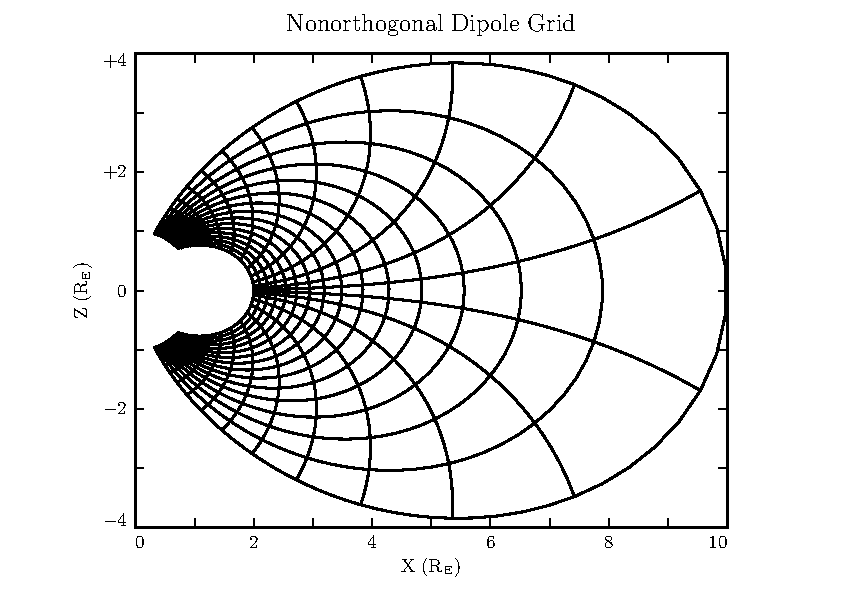
\includegraphics[width=\textwidth]{figures/fig_grid.pdf}
    \caption{
        The model's nonorthogonal grid accommodates both a field-aligned geometry and a constant-height ionospheric boundary. Every fifth point is shown in each direction. The high concentration of grid points near Earth's equator is a consequence of the coordinate system, which converges at the equatorial ionosphere. Earth (not shown) is centered at the origin with unit radius.
    }
    \label{fig_grid}
    \end{center}
\end{figure}

Here, $R$ is the geocentric radius of the ionospheric boundary, taken to be at $R_E + \SI{100}{\km}$, $\theta_0$ is the invariant colatitude, and $r$, $\theta$, and $\phi$ are the usual spherical coordinates.

A thorough discussion of these coordinates, and explicit forms for the resulting basis vectors and metric tensor components can be found in \citep{lysak_2004}. At present, it's sufficient to note that the coordinates are nonorthogonal, and thus have covariant and contravariant basis vectors (${\underline{e}_i \equiv \frac{\partial u^i}{\partial \underline{r}}}$ and ${\underline{e}^i \equiv \frac{\partial \underline{r}}{\partial u^i}}$ respectively) that do not line up with one another. However, both the covariant and contravariant basis vectors are important to the model.

The basis vectors $\underline{e}^1$, $\underline{e}^2$, and $\underline{e}_3$ are parallel to the usual dipole coordinates, as shown in \cref{to_dipole}, which is the natural basis for the conductivity and electric tensors.
\begin{linenomath*}
\begin{align}
    \label{to_dipole}
    \underline{e}^1 &\parallel \hat{x} &
    \underline{e}^2 &\parallel \hat{y} &
    \underline{e}_3 &\parallel \hat{z}
\end{align}
\end{linenomath*}

Where $\hat{z}$ lies along the magnetic field, $\hat{y}$ is azimuthally eastward, and $\hat{x} \equiv \hat{y} \times \hat{z}$ points radially outward at the equator.

In addition, at the ionospheric boundary, $\underline{e}_1$, $\underline{e}_2$, and $\underline{e}^3$ are parallel to the spherical unit vectors:
\begin{linenomath*}
\begin{align}
  \underline{e}_1 &\parallel \hat{\theta} &
  \underline{e}_2 &\parallel \hat{\phi} &
  \underline{e}^3 &\parallel \hat{r}
\end{align}
\end{linenomath*}


As a result, Tuna's grid is aligned everywhere to the zeroth-order dipole magnetic field, while also supporting a fixed-altitude ionospheric boundary.

The results shown in the present work use a grid of 150 values in $u^1$ (150 field lines) and 350 values in $u^3$ (350 grid points per field line). Spacing is on the order of \SI{10}{\km} near the ionosphere and \SI{1000}{\km} at the equator of the outermost field line. The inner boundary is placed at $L = 2$, and the outer boundary at $L = 10$. The time step is determined from the smallest Alfve\'n crossing time, scaled down by a Courant factor of \num{0.1}. Typically, $\delta \! t \sim \SI{10}{\us}$.

% ======================================================================

Like the similar models of \citep{lysak_2013} and \citep{waters_2013}, Tuna can be driven via compression of the simulation's outer boundary -- typically taken as a proxy for solar wind activity. However, the shear and compressional Alfve\'n modes decouple at high $m$, preventing such waves from propagating across magnetic field lines. In order to model noncompressional Pc4 activity at $L\sim5$, it's necessary to inject energy at $L\sim5$.

To this end, Tuna also allows simulations to be driven via modulation of the ring current, a proxy for substorm injection events. For the runs shown, the driving current is spread over a cross section of $\sim\SI{1}{R_E}^2$, centered just outside the plasmapause and just off the equator. In effect, the energy is delivered into a first-harmonic poloidal wave.

The magnitude of the driving current is estimated from a discrete Fourier transform of the Sym-H storm index during the June 1, 2013 storm. Sym-H is tabulated once per minute, which is too slow to capture activity in the Pc4 band directly. However, a fit of the pink noise spectrum, shown in \cref{fig_symh}, suggests that activity in the Pc4 range could plausibly give rise to a field at Earth's surface on the order of \SI{e-2}{\nT}.

This corresponds to a ring current perturbation on the order of \SI{1}{\mega\A}, or $\sim\SI{e-4}{\uA/\m\squared}$ spread over $\sim\SI{1}{\RE}^2$. For the runs shown in the present work, the driving current is azimuthally directed, and its magnitude varies sinusoidally.

\begin{figure}
    \begin{center}
    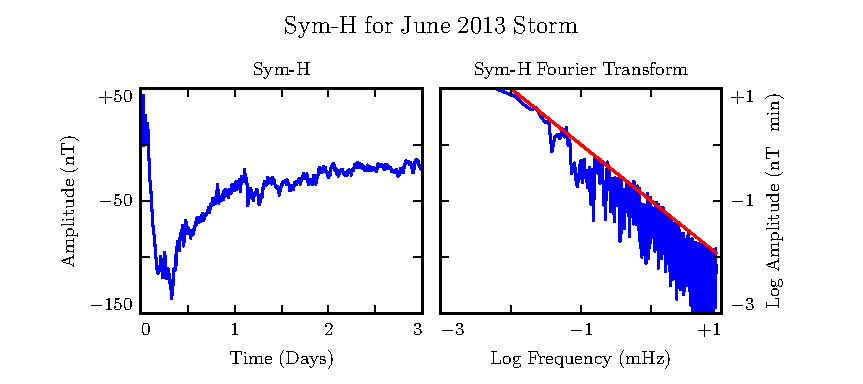
\includegraphics[width=\textwidth]{figures/fig_symh.pdf}
    \caption{
    Shown in red is $\frac{ \SI{0.1}{\nT} }{f}$. The vertical axis is scaled to inverse minutes. The width of the Pc4 frequency band (\SIrange{7}{25}{\mHz}) is about one inverse minute.
    }
    \label{fig_symh}
    \end{center}
\end{figure}

% ======================================================================

Mathematically, the driving current is introduced through an anomalous current term $\underline{J}$ in Amp\`ere's law, apart from the Ohmic current ${\underline{\underline{\sigma}} \cdot \underline{E}}$.

\begin{linenomath*}
\begin{align}
    \label{amp_law}
    \underline{\underline{\epsilon}} \cdot \frac{\partial}{\partial t} \underline{E} &= \frac{1}{\mu_0} \nabla \times \underline{B} - \underline{J}
      - \underline{\underline{\sigma}} \cdot \underline{E}
\end{align}
\end{linenomath*}

Because of the Ohmic current term, the electric field's time derivative in \cref{amp_law} depends on its own future value. This circular dependence is resolved using integrating factors. First, the expression is rewritten:
\begin{linenomath*}
\begin{align}
    \label{int_fac}
    \Big( \underline{\underline{\Omega}} + \underline{\underline{ \mathbb{I} }}\frac{\partial}{\partial t} \Big) \cdot
        \underline{E} &= \underline{\underline{V}}^2 \cdot \underline{F}
\end{align}
\end{linenomath*}

Where $\underline{\underline{ \mathbb{I} }}$ is the identity and $\underline{F}$, $\underline{\underline{V}}^2$, and $\underline{\underline{\Omega}}$ are shorthand:
\begin{linenomath*}
\begin{align}
    \underline{F} &\equiv \nabla \times \underline{B} - \mu_0 \underline{J} &
    \underline{\underline{V}}^2 &\equiv \frac{1}{\mu_0} \underline{\underline{\epsilon}}^{-1} &
    \underline{\underline{\Omega}} &\equiv \underline{\underline{\epsilon}}^{-1} \cdot \underline{\underline{\sigma}}
\end{align}
\end{linenomath*}

\cref{int_fac} is then solved by multiplying through by $\exp \left( \underline{\underline{\Omega}} \, t \right)$ (see \citep{hall_2015}), applying the product rule, and integrating over a time step $\delta \! t$.
\begin{linenomath*}
\begin{align}
    \label{amp_final}
    \underline{E} &\leftarrow \exp \left( -\underline{\underline{\Omega}} \, \delta \! t \right) \cdot \underline{E} +
        \delta \! t \, \exp \left( -\underline{\underline{\Omega}} \, \tfrac{\delta \! t}{2} \right) \cdot
        \underline{\underline{V}}^2 \cdot \underline{F}
\end{align}
\end{linenomath*}

Where $\leftarrow$ represents the assignment of a future value based on existing values. If $E$ and $F$ on the right hand side correspond to times $-\frac{\delta \! t}{2}$ and $0$ respectively, the value of $E$ on the left is at time $\frac{\delta \! t}{2}$.

\cref{amp_final} is evaluated by separating the exponential into its diagonal (Pedersen) and off-diagonal (Hall) terms. The Hall terms give a rotation matrix around the magnetic field line, coupling the poloidal and toroidal modes, consistent with \citep{hughes_1974}. Terms proportional to $\exp \left( - \frac{\sigma_0}{\epsilon_0}\delta \! t \right)$ are also present. However, $\frac{\sigma_0}{\epsilon_0}\delta \! t \gtrsim 1000$, so these terms are vanishingly small. As a result, parallel electric fields are taken to be uniformly zero.

Magnetic fields are simply advanced using Faraday's law:
\begin{linenomath*}
\begin{align}
    \label{far_law}
    \frac{\partial}{\partial t} \underline{B} &= - \nabla \times \underline{E}
\end{align}
\end{linenomath*}

For the sake of brevity, the present work does not expand the terms of \cref{amp_final,far_law} in the covariant basis. Those expressions can be found in \citep{mceachern_2016}.

% ======================================================================

Dirichlet and Neumann conditions are applied to the electric and magnetic fields respectively at the inner and outer boundaries. Results of the present work are robust under an exchange of the two.

Between the top of the neutral atmosphere and the bottom of the ionosphere, the model includes a thin, horizontal current sheet representing the ionosphere's $E$ layer\citep{lysak_2004}. By integrating Amp\`ere's law over the layer, it can be shown\citep{fujita_1988} that the horizontal electric field values at the edge of the grid are determined by the jump in the horizontal magnetic fields:
\begin{linenomath*}
\begin{align}
  \label{jump_condition}
  \underline{\underline{\Sigma}} \cdot \underline{E} &= \frac{1}{\mu_0} \,
    \displaystyle\lim_{\delta \! r \rightarrow 0} \, \bigg[ \, \hat{r} \times \underline{B}
    \, \bigg|^{R_I + \delta \! r}_{R_I - \delta \! r}
\end{align}
\end{linenomath*}

The atmospheric magnetic field is computed in terms of a scalar magnetic potential, $\Psi$, such that $\underline{B}=\nabla \Psi$. The neutral atmosphere is taken to be a perfect insulator, giving $\nabla \times \underline{B}=0$. Combined with $\nabla \cdot \underline{B}=0$ (per Maxwell's equations), this ensures that $\Psi$ satisfies Laplace's equation, $\nabla^2 \Psi = 0$, and thus can be written as a sum of harmonics\citep{jackson_1999}.
\begin{linenomath*}
\begin{align}
  \label{psi_expansion}
  \Psi &= \displaystyle\sum_\ell \left( a_\ell \, r^\ell +
    b_\ell \, r^{-\ell - 1} \right) Y_{\ell m}
\end{align}
\end{linenomath*}

Earth is taken to be a perfect conductor, so $B_r = \frac{\partial}{\partial r} \Psi = 0$ at the surface. In addition, the thin current sheet at the top of the atmosphere is taken to be horizontal, so the radial component of the magnetic field must be the same just above and just below it. Those two boundary conditions (combined with the harmonics' orthonormality) allow solutions for the coefficients $a_\ell$ and $b_\ell$, giving:
\begin{linenomath*}
\begin{align}
  \label{psi_final}
  \begin{split}
  \Psi_E &= \displaystyle\sum_\ell Y_{\ell m} \; \frac{R_I}{ \ell \, \left(\ell - 1\right) } \frac{ \left(2 \ell - 1\right) \, \lambda^\ell }{ 1 - \lambda^{2 \ell + 1} } B_r \cdot Y_{\ell m}^{-1} \\
  \Psi_I &= \displaystyle\sum_\ell Y_{\ell m} \; \frac{R_I}{ \ell \, \left(\ell - 1\right) } \frac{ \left(\ell - 1\right) + \ell \, \lambda^{2 \ell + 1} }{ 1 - \lambda^{2 \ell + 1} } B_r \cdot Y_{\ell m}^{-1}
  \end{split}
\end{align}
\end{linenomath*}

Where $\Psi_E$ and $\Psi_I$ are the values of $\Psi$ at $R_E$ (Earth's surface) and $R_I$ (The bottom of the ionosphere) respectively, $\lambda \equiv \frac{R_E}{R_I} \sim \num{0.975}$, and $B_r \cdot Y_{\ell m}^{-1} \equiv \displaystyle\sum_i B_r [i] \; Y_{\ell m}^{-1} \! [i]$.

Magnetic field values at the top of the atmosphere are used to compute electric field boundary conditions via \cref{jump_condition}. Those at Earth's surface are output, suitable for comparison with magnetometer data.







%% Example \citet and \citep:
%  ...as shown by \citet{Boug10}, \citet{Buiz07}, \citet{Fra10},
%  \citet{Ghel00}, and \citet{Leit74}.

%  ...as shown by \citep{Boug10}, \citep{Buiz07}, \citep{Fra10},
%  \citep{Ghel00, Leit74}.

%  ...has been shown \citep [e.g.,][]{Boug10,Buiz07,Fra10}.





% ######################################################################

\bibliography{bibliography.bib}


%Text here ===>>>

%%

%  Numbered lines in equations:
%  To add line numbers to lines in equations,
%  \begin{linenomath*}
%  \begin{equation}
%  \end{equation}
%  \end{linenomath*}



%% Enter Figures and Tables near as possible to where they are first mentioned:
%
% DO NOT USE \psfrag or \subfigure commands.
%
% Figure captions go below the figure.
% Table titles go above tables;  other caption information
%  should be placed in last line of the table, using
% \multicolumn2l{$^a$ This is a table note.}
%
%----------------
% EXAMPLE FIGURE
%
% \begin{figure}[h]
% \centering
% when using pdflatex, use pdf file:
% \includegraphics[width=20pc]{figsamp.pdf}
%
% when using dvips, use .eps file:
% \includegraphics[width=20pc]{figsamp.eps}
%
% \caption{Short caption}
% \label{figone}
%  \end{figure}
%
% ---------------
% EXAMPLE TABLE
%
% \begin{table}
% \caption{Time of the Transition Between Phase 1 and Phase 2$^{a}$}
% \centering
% \begin{tabular}{l c}
% \hline
%  Run  & Time (min)  \\
% \hline
%   $l1$  & 260   \\
%   $l2$  & 300   \\
%   $l3$  & 340   \\
%   $h1$  & 270   \\
%   $h2$  & 250   \\
%   $h3$  & 380   \\
%   $r1$  & 370   \\
%   $r2$  & 390   \\
% \hline
% \multicolumn{2}{l}{$^{a}$Footnote text here.}
% \end{tabular}
% \end{table}

%% SIDEWAYS FIGURE and TABLE
% AGU prefers the use of {sidewaystable} over {landscapetable} as it causes fewer problems.
%
% \begin{sidewaysfigure}
% \includegraphics[width=20pc]{figsamp}
% \caption{caption here}
% \label{newfig}
% \end{sidewaysfigure}
%
%  \begin{sidewaystable}
%  \caption{Caption here}
% \label{tab:signif_gap_clos}
%  \begin{tabular}{ccc}
% one&two&three\\
% four&five&six
%  \end{tabular}
%  \end{sidewaystable}

%% If using numbered lines, please surround equations with \begin{linenomath*}...\end{linenomath*}
%\begin{linenomath*}
%\begin{equation}
%y|{f} \sim g(m, \sigma),
%\end{equation}
%\end{linenomath*}

%%% End of body of article

%%%%%%%%%%%%%%%%%%%%%%%%%%%%%%%%
%% Optional Appendix goes here
%
% The \appendix command resets counters and redefines section heads
%
% After typing \appendix
%
%\section{Here Is Appendix Title}
% will show
% A: Here Is Appendix Title
%
%\appendix
%\section{Here is a sample appendix}

%%%%%%%%%%%%%%%%%%%%%%%%%%%%%%%%%%%%%%%%%%%%%%%%%%%%%%%%%%%%%%%%
%
% Optional Glossary, Notation or Acronym section goes here:
%
%%%%%%%%%%%%%%
% Glossary is only allowed in Reviews of Geophysics
%  \begin{glossary}
%  \term{Term}
%   Term Definition here
%  \term{Term}
%   Term Definition here
%  \term{Term}
%   Term Definition here
%  \end{glossary}

%
%%%%%%%%%%%%%%
% Acronyms
%   \begin{acronyms}
%   \acro{Acronym}
%   Definition here
%   \acro{EMOS}
%   Ensemble model output statistics
%   \acro{ECMWF}
%   Centre for Medium-Range Weather Forecasts
%   \end{acronyms}

%
%%%%%%%%%%%%%%
% Notation
%   \begin{notation}
%   \notation{$a+b$} Notation Definition here
%   \notation{$e=mc^2$}
%   Equation in German-born physicist Albert Einstein's theory of special
%  relativity that showed that the increased relativistic mass ($m$) of a
%  body comes from the energy of motion of the body—that is, its kinetic
%  energy ($E$)—divided by the speed of light squared ($c^2$).
%   \end{notation}




%%%%%%%%%%%%%%%%%%%%%%%%%%%%%%%%%%%%%%%%%%%%%%%%%%%%%%%%%%%%%%%%
%
%  ACKNOWLEDGMENTS
%
% The acknowledgments must list:
%
% •	All funding sources related to this work from all authors
%
% •	Any real or perceived financial conflicts of interests for any
%	author
%
% •	Other affiliations for any author that may be perceived as
% 	having a conflict of interest with respect to the results of this
% 	paper.
%
% •	A statement that indicates to the reader where the data
% 	supporting the conclusions can be obtained (for example, in the
% 	references, tables, supporting information, and other databases).
%
% It is also the appropriate place to thank colleagues and other contributors.
% AGU does not normally allow dedications.


\acknowledgments
 = enter acknowledgments here =


%% ------------------------------------------------------------------------ %%
%% Citations

% Please use ONLY \citet and \citep for reference citations.
% DO NOT use other cite commands (e.g., \cite, \citeyear, \nocite, \citealp, etc.).


%% Example \citet and \citep:
%  ...as shown by \citet{Boug10}, \citet{Buiz07}, \citet{Fra10},
%  \citet{Ghel00}, and \citet{Leit74}.

%  ...as shown by \citep{Boug10}, \citep{Buiz07}, \citep{Fra10},
%  \citep{Ghel00, Leit74}.

%  ...has been shown \citep [e.g.,][]{Boug10,Buiz07,Fra10}.



%%  REFERENCE LIST AND TEXT CITATIONS
%
% Either type in your references using
%
% \begin{thebibliography}{}
% \bibitem[{\textit{Kobayashi et~al.}}(2003)]{R2013} Kobayashi, T.,
% Tran, A.~H., Nishijo, H., Ono, T., and Matsumoto, G.  (2003).
% Contribution of hippocampal place cell activity to learning and
% formation of goal-directed navigation in rats. \textit{Neuroscience}
% 117, 1025--1035.
%
% \bibitem{}
% Text
% \end{thebibliography}
%
%%%%%%%%%%%%%%%%%%%%%%%%%%%%%%%%%%%%%%%%%%%%%%%
% Or, to use BibTeX:
%
% Follow these steps
%
% 1. Type in \bibliography{<name of your .bib file>}
%    Run LaTeX on your LaTeX file.
%
% 2. Run BiBTeX on your LaTeX file.
%
% 3. Open the new .bbl file containing the reference list and
%   copy all the contents into your LaTeX file here.
%
% 4. Run LaTeX on your new file which will produce the citations.
%
% AGU does not want a .bib or a .bbl file. Please copy in the contents of your .bbl file here.


%% After you run BibTeX, Copy in the contents of the .bbl file here:


%%%%%%%%%%%%%%%%%%%%%%%%%%%%%%%%%%%%%%%%%%%%%%%%%%%%%%%%%%%%%%%%%%%%%
% Track Changes:
% To add words, \added{<word added>}
% To delete words, \deleted{<word deleted>}
% To replace words, \replace{<word to be replaced>}{<replacement word>}
% To explain why change was made: \explain{<explanation>} This will put
% a comment into the right margin.

%%%%%%%%%%%%%%%%%%%%%%%%%%%%%%%%%%%%%%%%%%%%%%%%%%%%%%%%%%%%%%%%%%%%%
% At the end of the document, use \listofchanges, which will list the
% changes and the page and line number where the change was made.

% When final version, \listofchanges will not produce anything,
% \added{<word or words>} word will be printed, \deleted{<word or words} will take away the word,
% \replaced{<delete this word>}{<replace with this word>} will print only the replacement word.
%  In the final version, \explain will not print anything.
%%%%%%%%%%%%%%%%%%%%%%%%%%%%%%%%%%%%%%%%%%%%%%%%%%%%%%%%%%%%%%%%%%%%%

%%%
\listofchanges
%%%

\end{document}

%%%%%%%%%%%%%%%%%%%%%%%%%%%%%%%%%%%%%
%% Supporting Information
%% (Optional) See AGUSuppInfoSamp.tex/pdf for requirements
%% for Supporting Information.
%%%%%%%%%%%%%%%%%%%%%%%%%%%%%%%%%%%%%



%%%%%%%%%%%%%%%%%%%%%%%%%%%%%%%%%%%%%%%%%%%%%%%%%%%%%%%%%%%%%%%

More Information and Advice:

%% ------------------------------------------------------------------------ %%
%
%  SECTION HEADS
%
%% ------------------------------------------------------------------------ %%

% Capitalize the first letter of each word (except for
% prepositions, conjunctions, and articles that are
% three or fewer letters).

% AGU follows standard outline style; therefore, there cannot be a section 1 without
% a section 2, or a section 2.3.1 without a section 2.3.2.
% Please make sure your section numbers are balanced.
% ---------------
% Level 1 head
%
% Use the \section{} command to identify level 1 heads;
% type the appropriate head wording between the curly
% brackets, as shown below.
%
%An example:
%\section{Level 1 Head: Introduction}
%
% ---------------
% Level 2 head
%
% Use the \subsection{} command to identify level 2 heads.
%An example:
%\subsection{Level 2 Head}
%
% ---------------
% Level 3 head
%
% Use the \subsubsection{} command to identify level 3 heads
%An example:
%\subsubsection{Level 3 Head}
%
%---------------
% Level 4 head
%
% Use the \subsubsubsection{} command to identify level 3 heads
% An example:
%\subsubsubsection{Level 4 Head} An example.
%
%% ------------------------------------------------------------------------ %%
%
%  IN-TEXT LISTS
%
%% ------------------------------------------------------------------------ %%
%
% Do not use bulleted lists; enumerated lists are okay.
% \begin{enumerate}
% \item
% \item
% \item
% \end{enumerate}
%
%% ------------------------------------------------------------------------ %%
%
%  EQUATIONS
%
%% ------------------------------------------------------------------------ %%

% Single-line equations are centered.
% Equation arrays will appear left-aligned.

Math coded inside display math mode \[ ...\]
 will not be numbered, e.g.,:
 \[ x^2=y^2 + z^2\]

 Math coded inside \begin{equation} and \end{equation} will
 be automatically numbered, e.g.,:
 \begin{equation}
 x^2=y^2 + z^2
 \end{equation}


% To create multiline equations, use the
% \begin{eqnarray} and \end{eqnarray} environment
% as demonstrated below.
\begin{eqnarray}
  x_{1} & = & (x - x_{0}) \cos \Theta \nonumber \\
        && + (y - y_{0}) \sin \Theta  \nonumber \\
  y_{1} & = & -(x - x_{0}) \sin \Theta \nonumber \\
        && + (y - y_{0}) \cos \Theta.
\end{eqnarray}

%If you don't want an equation number, use the star form:
%\begin{eqnarray*}...\end{eqnarray*}

% Break each line at a sign of operation
% (+, -, etc.) if possible, with the sign of operation
% on the new line.

% Indent second and subsequent lines to align with
% the first character following the equal sign on the
% first line.

% Use an \hspace{} command to insert horizontal space
% into your equation if necessary. Place an appropriate
% unit of measure between the curly braces, e.g.
% \hspace{1in}; you may have to experiment to achieve
% the correct amount of space.


%% ------------------------------------------------------------------------ %%
%
%  EQUATION NUMBERING: COUNTER
%
%% ------------------------------------------------------------------------ %%

% You may change equation numbering by resetting
% the equation counter or by explicitly numbering
% an equation.

% To explicitly number an equation, type \eqnum{}
% (with the desired number between the brackets)
% after the \begin{equation} or \begin{eqnarray}
% command.  The \eqnum{} command will affect only
% the equation it appears with; LaTeX will number
% any equations appearing later in the manuscript
% according to the equation counter.
%

% If you have a multiline equation that needs only
% one equation number, use a \nonumber command in
% front of the double backslashes (\\) as shown in
% the multiline equation above.

% If you are using line numbers, remember to surround
% equations with \begin{linenomath*}...\end{linenomath*}

%  To add line numbers to lines in equations:
%  \begin{linenomath*}
%  \begin{equation}
%  \end{equation}
%  \end{linenomath*}
